
%(BEGIN_QUESTION)
% Copyright 2007, Tony R. Kuphaldt, released under the Creative Commons Attribution License (v 1.0)
% This means you may do almost anything with this work of mine, so long as you give me proper credit

We know that a simple one-resistor, one-capacitor circuit mimics the behavior of a single-order process:

$$\includegraphics[width=15.5cm]{i01681x01.eps}$$

Modify this resistor-capacitor circuit to have a {\it second-order} response, in order to mimic a second-order process.

\vskip 10pt

Now, explain what it is about this process that makes it second-order:

$$\includegraphics[width=15.5cm]{i01681x03.eps}$$

\underbar{file i01681}
%(END_QUESTION)





%(BEGIN_ANSWER)

$$\includegraphics[width=15.5cm]{i01681x02.eps}$$

The mass has thermal ``capacitance'' in that it stores heat energy, and the insulating box enclosing the mass offers ``resistance'' to the flow of heat energy to or from the mass.  This mass-in-box system comprises one order of dynamic lag.  The oven itself, with its own mass (metal shell) and insulation (air space within), comprises the second order of dynamic lag, making this a second-order system.

%(END_ANSWER)





%(BEGIN_NOTES)

Since a second-order process is one with two storage (``capacitive'') elements and two limiting (``resistive'') elements cascaded, all we need to do to our RC circuit is add another stage of resistance and capacitance as such:

%INDEX% Control, basics: second-order process (modeled by an RC circuit)

%(END_NOTES)


